As already mentioned, the behavior of the time varying electromagnetic field in free space is governed by the microscopic variant of Maxwell equations (\ref{1.1} - \ref{1.4}). A typical numerical technique to resolve the Maxwell's equations with respect to time is finite-difference time-domain method (FDTD), because it is probably the simplest technique in terms of the implementation.

The vector components of the fields $ \vec{E}_{ijk}^{\,n} $ and $ \vec{B}_{ijk}^{\,n} $ are spatially staggered about rectangular cells of the computational grid,
\begin{equation}
\label{3.1.1.4}
\vec{E}_{ijk}^{\,n} \rightarrow \left[\left(E_{x}\right)^{n}_{i,\: j + 1/2,\: k + 1/2}, \left(E_{y}\right)^{n}_{i + 1/2,\: j,\: k + 1/2}, \left(E_{z}\right)^{n}_{i + 1/2,\: j + 1/2,\: k} \right],
\end{equation}
\begin{equation}
\label{3.1.1.5}
\vec{B}_{ijk}^{\,n} \rightarrow \left[\left(B_{x}\right)^{n}_{i + 1/2,\: j,\: k}, \left(B_{y}\right)^{n}_{i,\: j + 1/2,\: k}, \left(B_{z}\right)^{n}_{i,\: j,\: k + 1/2} \right].
\end{equation}
This scheme, which has proven to be very robust, is now known as a Yee lattice \cite{yee}. The illustration of a standard Cartesian Yee cell used for FDTD is shown in Figure \ref{3.1.1.14}. Components of the current density $ \vec{J}_{ijk}^{\:n} $ are defined in the same way as the components of $ \vec{E}_{ijk}^{\:n} $, charge density $ \rho_{ijk}^{\:n} $ is defined in the middle of the cell,
\begin{equation}
\vec{J}_{ijk}^{\,n} \rightarrow \left[\left(J_{x}\right)^{n}_{i,\: j + 1/2,\: k + 1/2}, \left(J_{y}\right)^{n}_{i + 1/2,\: j,\: k + 1/2}, \left(J_{z}\right)^{n}_{i + 1/2,\: j + 1/2,\: k} \right],
\end{equation}
\begin{equation}
\rho_{ijk}^{\,n} \rightarrow \rho_{i + 1/2,\: j + 1/2,\: k + 1/2}^{\,n}.
\end{equation}

For marching in time a leap-frog scheme is used, thus discretized Maxwell's equations \ref{1.1} - \ref{1.4} have the following form,
\begin{equation}
\label{3.1.1.6}
\nabla^{+} \cdot \vec{E}_{ijk}^{\,n} = \frac{\rho_{ijk}^{\,n}}{\varepsilon_0},
\end{equation}
\begin{equation}
\label{3.1.1.15}
\nabla^{-} \cdot \vec{B}_{ijk}^{\,n + 1/2} = 0,
\end{equation}
\begin{equation}
\label{3.1.1.16}
\frac{1}{c^{2}} \frac{\vec{E}_{ijk}^{\,n + 1} - \vec{E}_{ijk}^{\,n}}{\Delta t} = \nabla^{+} \times \vec{B}_{ijk}^{\,n + 1/2} - \mu_{0} \vec{J}_{ijk}^{\,n + 1/2},
\end{equation}
\begin{figure}[t]
	\centering
	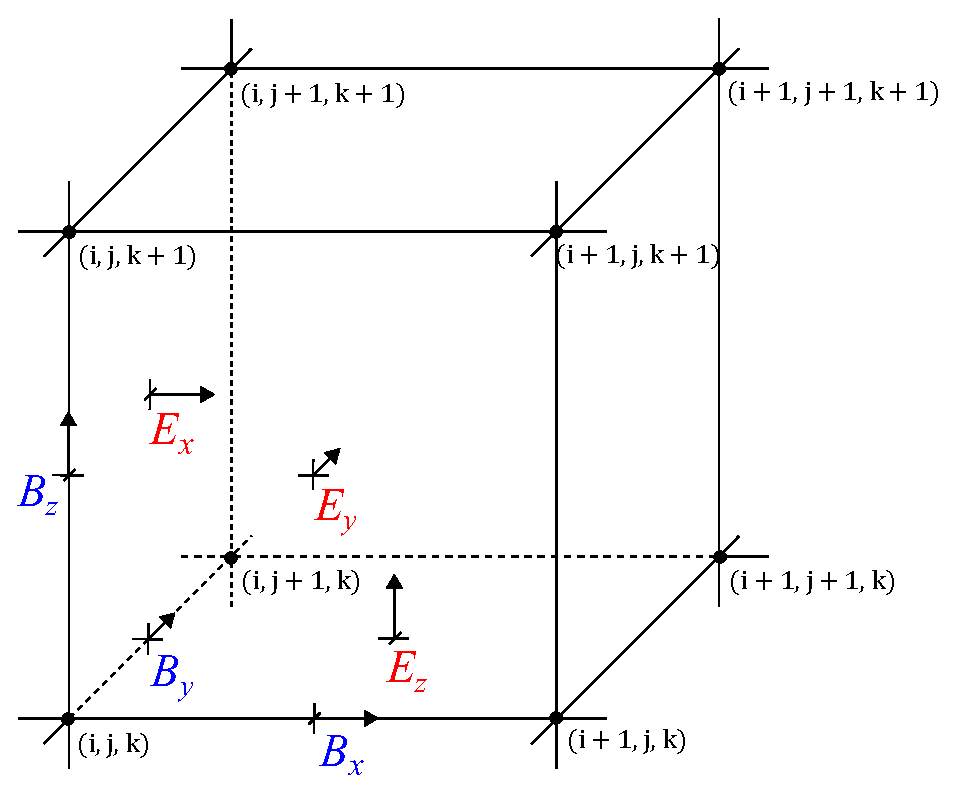
\includegraphics[width=0.355\paperwidth]{./img/YEE/yee.eps}
	\caption{Standard Cartesian Yee cell used for FDTD method}
	\label{3.1.1.14}
\end{figure}
\begin{equation}
\label{3.1.1.7}
\frac{\vec{B}_{ijk}^{\,n + 1/2} - \vec{B}_{ijk}^{\,n - 1/2}}{\Delta t} = -\nabla^{-} \times \vec{E}_{ijk}^{\,n}.
\end{equation}
Notice that this scheme achieves second-order accuracy in both, space and time. Discrete operators $ \left(\nabla^{+}\right) $ and $ \left(\nabla^{-}\right) $ used in \ref{3.1.1.6} - \ref{3.1.1.7} act on a scalar field $ f_{i j k} $ as follows,
\begin{equation}
\label{3.1.1.8}
\nabla^{+} f_{i j k} = \left(\frac{f_{i + 1,\: j,\: k} - f_{i,\: j,\: k}}{\Delta x}, \frac{f_{i,\: j + 1,\: k} - f_{i,\: j,\: k}}{\Delta y}, \frac{f_{i,\: j,\: k + 1} - f_{i,\: j,\: k}}{\Delta z} \right), 
\end{equation}
\begin{equation}
\label{3.1.1.9}
\nabla^{-} f_{i j k} = \left(\frac{f_{i,\: j,\: k} - f_{i - 1,\: j,\: k}}{\Delta x}, \frac{f_{i,\: j,\: k} - f_{i,\: j - 1,\: k}}{\Delta y}, \frac{f_{i,\: j,\: k} - f_{i,\: j,\: k - 1}}{\Delta z} \right).
\end{equation}
These operators have the following properties,
\begin{equation}
\label{3.1.1.10}
\nabla^{-} \cdot \nabla^{-} \times = \nabla^{+} \cdot \nabla^{+} \times = 0, \qquad \nabla^{-} \cdot \nabla^{+} = \nabla^{+} \cdot \nabla^{-} = \Delta^{\pm}.
\end{equation}
Symbol $ \Delta^{\pm} $ stands for the discrete Laplace operator in central differences,
\begin{equation}
\label{3.1.1.11}
\Delta^{\pm} f_{i, j, k} = \frac{f_{i - 1, j, k} + 2 f_{i, j, k} + f_{i + 1, j, k}}{\Delta x^{2}} + \frac{f_{i, j - 1, k} + 2 f_{i, j, k} + f_{i, j + 1, k}}{\Delta y^{2}} + \frac{f_{i, j, k - 1} + 2 f_{i, j, k} + f_{i, j, k + 1}}{\Delta z^{2}}.
\end{equation}

Before trying to find the solution of discretized Maxwell equations \ref{3.1.1.6} - \ref{3.1.1.7}, one must realize that this system of equations is not independent. In the three-dimensional case, there are eight first-order differential equations, but only six unknown vector components. Acting on the equations \ref{3.1.1.16} and \ref{3.1.1.7} by operators $ \left(\nabla^{-}\cdot\right) $ and $ \left(\nabla^{+}\cdot\right) $, respectively, one obtains
\begin{equation}
\label{3.1.1.12}
\frac{\nabla^{-} \cdot \vec{B}_{ijk}^{\,n + 1/2} - \nabla^{-} \cdot \vec{B}_{ijk}^{\,n - 1/2}}{\Delta t} = 0,
\end{equation}
\begin{equation}
\label{3.1.1.13}
\frac{\rho_{ijk}^{\,n + 1} - \rho_{ijk}^{\,n}}{\Delta t} + \nabla^{+} \cdot \vec{J}_{ijk}^{\,n + 1/2} = 0.
\end{equation}
It means that it is possible to solve only the equations \ref{3.1.1.16} and \ref{3.1.1.7}, while the divergence equations \ref{3.1.1.6}, \ref{3.1.1.15} can be considered as the initial conditions. Note that in this case, the continuity equation in the finite differences (\ref{3.1.1.13}) has to be fulfilled.